\lab{The Arnoldi Iteration}{The Arnoldi Iteration}
\label{lab:kry_arnoldi}

\objective{Use Krylov subspaces to find eigenvalues of extremely large matrices.}

One of the biggest difficulties in computational linear algebra is the amount of memory needed to store a large matrix and the amount of time needed to read its entries.
Methods using Krylov subspaces avoid this difficulty by studying how a matrix acts on vectors, making it unnecessary in many cases to create the matrix itself.

The \emph{Arnoldi iteration} is an algorithm for finding an orthonormal basis of a Krylov subspace.
One of its strengths is it can run on any linear operator without knowing the operator's underlying matrix representation.
The outputs of the Arnoldi algorithm can be used to approximate the eigenvalues of the matrix of the linear operator.

\section*{Krylov Subspaces} % =================================================

The order-$N$ Krylov subspace of $A$ generated by $\x$ is
\[
\mathcal{K}_n(A, \x) =\text{span} \{\x, A\x, A^2\x, \ldots, A^{n-1}\x\}.
\]
If the vectors $\{\x, A\x, A^2\x, \ldots, A^{n-1}\x\}$ are linearly independent, then they form a basis for $\mathcal{K}_n(A,\x)$.
However, this basis is usually far from orthogonal, and hence computations using this basis will likely be ill-conditioned.

\section*{The Arnoldi Iteration Algorithm} % ==================================

One way to find an orthonormal basis for $\mathcal{K}_n(A,\x)$ is to use the modified Gram-Schmidt algorithm from Lab \ref{lab:QRdecomp} on the set $\{\x, A\x, A^2\x, \ldots, A^{n-1}\x\}$.
The Arnold iteration does this more efficiently by integrating the creation of $\{\x, A\x, A^2\x, \ldots, A^{n-1}\x\}$ with the modified Gram-Schmidt algorithm. It returns an orthonormal basis for $\mathcal{K}_n(A,\x)$. This algorithm is described in Algorithm \ref{alg:arnoldi_iteration}.

\begin{comment}
Before discussing the specific uses of the Krylov subspace in linear systems and eigenvalue problems, let us address a very
practical concern: how can we best compute a basis for the Krylov subspace? The obvious answer is simply to
calculate the vectors $x, Ax, A^2x, \ldots, A^{N-1} x$, which we can accomplish using only matrix-vector multiplication.
Straightforward though this may be, there is a major problem: $A^n x$ tends to converge to a dominant eigenvector of $A$
as $n$ gets large, and consequently these vectors become nearly parallel. Thus, the basis $\{x, Ax, A^2x, \ldots, A^{N-1} x\}$
is far from orthogonal, and matrix computations associated with this basis will likely be ill-conditioned and prone to
numerical instability. To redress this problem, we may think to apply the Gram-Schmidt orthogonalization process to the
basis, obtaining an orthonormal basis for the Krylov subspace that enjoys much better numerical properties. This turns out to
be a useful thought, and is the basis for the Arnoldi iteration.

You may recall from lab \ref{lab:QRdecomp} that the Modified Gram-Schmidt algorithm allows us to find an increasing number of orthogonal
vectors but does not require that we run the algorithm to its completion to find a full basis.
Our goal is to find an orthonormal set of vectors $q_1,\ldots,q_N$ having the same span as $x, Ax, A^2x, \ldots, A^{N-1} x$.
We start
 things off by setting
\[
q_1 = \frac{x}{\|x\|_2}.
\]
Now, assuming we have obtained $q_1,\ldots,q_n$, we obtain $q_{n+1}$ by projecting $A q_n$ onto the previous vectors,
subtracting out these projections, and then normalizing. To make this more precise, let $h_{i,n} = \langle q_i, A q_n\rangle$
for $i = 1,\ldots, n$. Subtract out these projections by calculating
\[
p_{n+1} = A^n x - \sum_{i=1}^n h_{i,n}q_i.
\]
Define $h_{n+1,n} = \|p_{n+1}\|_2$, and normalize $p_{n+1}$ by calculating
\[
q_{n+1} = \frac{p_{n+1}}{h_{n+1,n}},
\]
our next basis vector. This procedure is outlined (in slightly more Python-friendly notation) in Algorithm \ref{alg:arnoldi_iteration}.

Perhaps you noticed a slight discrepancy between the Arnoldi iteration as described above, and the usual Gram-Schmidt procedure.
Specifically, you might have expected to compute $q_{n+1}$ by projecting $A^n x$, rather than $A q_n$, onto the previous vectors.
Thankfully, it is straightforward to show that our algorithm produces a valid orthonormal basis for the Krylov subspace,
despite this difference. And because of this detail, we do not need to compute and store the original Krylov basis
$x, Ax, \ldots, A^{N-1}x$.
Additionally, each iteration only requires one matrix-vector calculation, and the individual entries in $A$ are never
referenced or modified. Thus, even if the matrix $A$ is very large in theory, as long as we have a reasonably efficient
subroutine to calculate $Ax$ for any vector $x$, the Arnoldi iteration is computationally tractable.

This algorithm produces an orthonormal basis $q_1,\ldots,q_N$ for the order-$N$ Krylov subspace generated by $A$ and $x$, as well
as a collection of numbers $h_{i,j}$. If we define a matrix $H_N$ whose $i,j$'th entry is $h_{i,j}$ for $i \leq j+1$ and
is $0$ otherwise, we now have an upper Hessenberg matrix.
Recall that an upper Hessenberg matrix has the property that all entries below the first subdiagonal
are equal to zero. Any square matrix is unitarily similar to an upper Hessenberg matrix. Dealing with a Hessenberg matrix is
often more convenient than dealing with a general matrix, especially when it comes to finding eigenvalues or solving systems
of equations, since efficient algorithms designed for these types of matrices exist.
It turns out that there is a Hessenberg factorization of $A$, given by
\[
A  = QHQ^*,
\]
where $Q$ is a unitary matrix and $H$ is upper Hessenberg such that the first $N$ columns of $Q$ are $q_1,\ldots,q_N$, and
the upper left $N \times N$ submatrix of $H$ is equal to $H_N$. Hence, the Arnoldi iteration provides a connection between
the Krylov subspace and the Hessenberg factorization of a matrix. Each step in the Arnoldi iteration can be thought of as computing
another step in the Hessenberg reduction of $A$. Each $H_N$ is really just the $N \times N + 1$ upper-left block of $H$.
Solving eigenvalue problems or systems of equations for
a general square matrix can thus be reduced, via Arnoldi iteration, to solving these problems for a Hessenberg matrix,
a much easier task.

At this point, we can view the Arnoldi iteration as a means to compute an orthonormal basis for a Krylov subspace, or
alternatively, to compute a partial Hessenberg factorization of a matrix.
But in Lab \ref{lab:Canonical_Transformations}, we discussed how orthogonal transformations can be used to transform a matrix to Upper
Hessenberg form.
We were able to find the eigenvalues of such Upper Hessenberg matrices in Lab \ref{lab:EigSolve}.
So what have we really gained by this new approach?
These previous approaches were based on matrix-matrix multiplication and required us to manipulate individual entries of the matrix.
The Arnoldi iteration avoids this and relies only on our ability to calculate matrix-vector multiplication.
Further, our present approach will allow us to compute only a partial Hessenberg factorization. This is advantageous when, as
is often the case, the behavior and properties of a matrix can be well-approximated by only a small portion of its Hessenberg
form.
\end{comment}

\begin{algorithm}
\begin{algorithmic}[1]
\Procedure{Arnoldi}{$\b, A, k, tol$}
	\State $Q \gets \allocate{\size{\b}}{k+1}$			\Comment{Some initialization steps}
	\State $H \gets \zeros{ k+1}{ k}$
	\State $Q[:,0] \gets \b/\norm{\b}_2$
	\For{$j=0\ldots k-1$}							\Comment{Perform the actual iteration.}
		\State $Q[:,j+1] \gets AQ[:,j]$
		\For{$i=0\ldots j$}					\Comment{Modified Gram-Schmidt.}
			\State $H[i,j] \gets Q[:,i]\trp Q[:,j+1]$
			\State $Q[:,j+1] \gets Q[:,j+1] - H[i,j] Q[:,i]$
		\EndFor
		\State $H[j+1,j] \gets \norm{Q[:,j+1]}_2$			\Comment{Set subdiagonal element of $H$.}
            \If{$|H[j+1,j]|<tol$}					\Comment{Stop if $\norm{Q[:,j+1]}_2$ is too small.}
			\State \pseudoli{return} $H[:j+1,:j+1]$, $Q[:,:j+1]$
		\EndIf
		\State $Q[:,j+1] \gets Q[:,j+1]/H[j+1,j]$				\Comment{Normalize $\q_{j+1}$.}
	\EndFor
	\State \pseudoli{return} $H[:-1, :]$, $Q$			\Comment{Return $H_{k}$.}
\EndProcedure
\end{algorithmic}
\caption{The Arnoldi Iteration. This algorithm accepts a square matrix $A$ and starting vector $\b$. It iterates $k$ times or until the norm of the next vector in the iteration is less than $tol$.
The algorithm returns upper Hessenberg $H$ and orthonormal $Q$ such that $H = Q^{\mathsf{H}}AQ$.}
\label{alg:arnoldi_iteration}
\end{algorithm}

In Algorithm \ref{alg:arnoldi_iteration}, $k$ is the number of times we multiply by $A$.
This will result in an order-$k+1$ Krylov subspace.

Something perhaps unexpected happens in the Arnoldi iteration if the starting vector $\x$ is an eigenvector of $A$.
If the corresponding eigenvalue is $\lambda$, then by definition $\mathcal{K}_k(A, \x)=\text{span}\{\x, \lambda \x, \lambda^2\x, \ldots, \lambda^k \x\}$, which is equal to the span of $\x$.
Let us trace through Algorithm \ref{alg:arnoldi_iteration} in this case. We will use $\q_i$ to denote the $i^{th}$ column of $Q$.

In line 4 we normalize $\x$, setting $\q_1 = \x/\|\x\|$.
In line 6 we set $\q_2 = A\q_1 = \lambda \q_1$.
Then in line 8
\[
H_{1,1} = \langle \q_1, \q_2 \rangle = \langle \q_1, \lambda \q_1 \rangle = \lambda \langle \q_1, \q_1 \rangle = \lambda,
\]
so in line 9 we subtract $\lambda \q_1$ from $\q_2$, ending with $\q_2=0$.

The vector $\q_2$ is supposed to be the next vector in the orthonormal basis for $\mathcal{K}_k(A, \x)$, but since it is 0, it is not linearly independent of $\q_1$. In fact, $\q_1$ already spans $\mathcal{K}_k(A, \x)$.
Hence, when in line 11 we find that the norm of $\q_2$ is zero (or close to it, allowing for numerical error), we terminate the algorithm early, returning the $1\times 1$ matrix $H = H_{1, 1}=\lambda$ and the $n\times 1$ matrix $Q = \q_1$.

A similar phenomenon may occur if the starting vector $\x$ is contained in a proper invariant subspace of $A$.

\section*{Arnoldi Iteration on Linear Operators} % ============================

A major strength of the Arnoldi Iteration is that it can run on a linear operator, even without knowing the matrix representation of the operator. If $A_{mul}$ is some linear function, then we can modify the pseudocode above by replacing $AQ[:,j]$ with $A_{mul}(Q[:,j])$. This will make it possible to find the eigenvalues of an arbitrary linear transformation. We will use this method in the problem below.

\begin{problem}\label{prob:arnoldi}
Using Algorithm \ref{alg:arnoldi_iteration}, complete the following Python function that performs the Arnoldi iteration.
Write this function so that it can run on complex arrays.

\begin{lstlisting}
def arnoldi(b, Amul, k, tol=1e-8):
    """Perform `k' steps of the Arnoldi iteration on the linear operator
    defined by `Amul', starting with the vector 'b'.

    Inputs:
        b (ndarray): The starting vector for the iteration.
        Amul (function): A function handle that describes a linear operator.
        k (int): The number of times to perform the iteration.
        tol (float): Stop iterating if the next vector in the iteration has
            norm less than `tol'. Defaults to 1e-8.

    Returns:
        H_n (ndarray)
        Q_n (ndarray)
            The number n will equal k, unless the algorithm terminated early,
            in which case n will be less than k.

    Examples:
        >>> A = np.array([[1,0,0],[0,2,0],[0,0,3]])
        >>> Amul = lambda x: A.dot(x)
        >>> H, Q = arnoldi(np.array([1,1,1]), Amul, 3)
        >>> np.allclose(H, np.conjugate(Q.T).dot(A).dot(Q) )
        True

        >>> H, Q = arnoldi(np.array([1,0,0]), Amul, 3)
        >>> H
        array([[ 1.+0.j]])
        >>> np.conjugate(Q.T).dot(A).dot(Q)
        array([[ 1.+0.j]])
    """
\end{lstlisting}

Hints:
\begin{enumerate}
\item Since \li{H} and \li{Q} will eventually hold complex numbers, initialize them as complex arrays (e.g., \li{A = np.empty((3,3), dtype=np.complex128)}).
\item Remember to use complex inner products.
\item This function can be tested on a matrix A by passing in \li{A.dot} for \li{Amul}.
\end{enumerate}
\end{problem}

\section*{Finding Eigenvalues Using Arnoldi Iteration} % ======================

Let $A$ be an $n \times n$ matrix.
Let $Q_k$ be the matrix whose columns $\q_1, \ldots, \q_k$ are the orthonormal basis for $\mathcal{K}_m(A, \x)$ generated by the Arnoldi algorithm, and
let $H_k$ be the $k\times k$ upper Hessenburg matrix defined at the $k^{th}$ stage of the algorithm.
Then these matrices satisfy
\begin{equation}\label{equ:hqa}
H_k = Q_k^{\mathsf H} A Q_k.
\end{equation}
If $k<n$, then $H_k$ is a low-rank approximation to $A$.
We may use its eigenvalues as approximations to the eigenvalues of $A$.
The eigenvalues of $H_k$ are called \emph{Ritz values}, and in fact they converge quickly to the largest eigenvalues of $A$.

\begin{problem}\label{prob:ritz}
Finish the following function that computes the Ritz values of a matrix.

\begin{lstlisting}
def ritz(Amul, dim, k, iters):
    """Find `k' Ritz values of the linear operator defined by `Amul'.

    Inputs:
        Amul (function): A function describing a linear operator on R^(dim).
        dim (int): The dimension of the space on which `Amul' acts.
        k (int): The number of Ritz values to return.
        iters (int): The number of times to perform the Arnoldi iteration.
            Must be between `k' and `dim'.

    Returns:
        ((k,) ndarray): `k' Ritz values of the operator defined by `Amul.'
    """
\end{lstlisting}
\end{problem}

One application of the Arnoldi iteration is to find the eigenvalues of linear operators that are too large to store in memory.
For example, if an operator acts on $\mathbb{C}^{2^{20}}$, then its matrix representation contains $2^{40}$ complex values.
Storing such a matrix would require 64 terabytes of memory!

An example of such an operator is the Fast Fourier Transform, cited by SIAM as one of the top algorithms of the century \cite{Cipra2000}.
The Fast Fourier Transform is used ubiquitously in the field of signal processing.

\begin{problem}
\label{prob:fourier_eigs}
The four largest eigenvalues of the Fast Fourier Transform are known to be $\{ -\sqrt{N}, \sqrt{N}, -i\sqrt{N}, i\sqrt{N} \}$ where $N$ is the dimension of the space on which the transform acts.
Use your function \li{ritz()} from Problem \ref{prob:ritz} to approximate the eigenvalues of the Fast Fourier Transform.
Set \li{k} to be 10 and set \li{dim} to be $2^{20}$.
For the argument \li{Amul}, use the \li{fft} function from \li{scipy.fftpack}.
\end{problem}

The Arnoldi iteration for finding eigenvalues is implemented in a Fortran library called ARPACK.
SciPy interfaces with the Arnoldi iteration in this library via the function \li{scipy.sparse.linalg.eigs()}.
This function has many more options than the implementation we wrote in Problem \ref{prob:ritz}.
In this example, the keyword argument \li{k=5} specifies that we want five Ritz values.
Note that even though this function comes from the \li{sparse} library in SciPy, we can still call it on regular NumPy arrays.

\begin{lstlisting}
>>> B = np.random.rand(10000).reshape(100, 100)
>>> sp.sparse.linalg.eigs(B, k=5, return_eigenvectors=False)
array([ -1.15577072-2.59438308j,  -2.63675878-1.09571889j,
        -2.63675878+1.09571889j,  -3.00915592+0.j        ,  50.14472893+0.j ])
\end{lstlisting}

\subsection*{Convergence} % ---------------------------------------------------

The Arnoldi method for finding eigenvalues quickly converges to eigenvalues whose magnitude is distinctly larger than the rest.
For example, matrices with random entries tend to have one eigenvalue of distinctly greatest magnitude.
Convergence of the Ritz values for such a matrix is plotted in Figure \ref{fig:arnoldi_random_val_conv}.

However, Ritz values converge more slowly for matrices with random eigenvalues.
Figure \ref{fig:arnoldi_random_eig_conv} plots convergence of the Ritz values for a matrix with eigenvalues uniformly distributed in $[0,1)$.

\begin{figure}
\centering
\begin{subfigure}[b]{.49\textwidth}
    \centering
    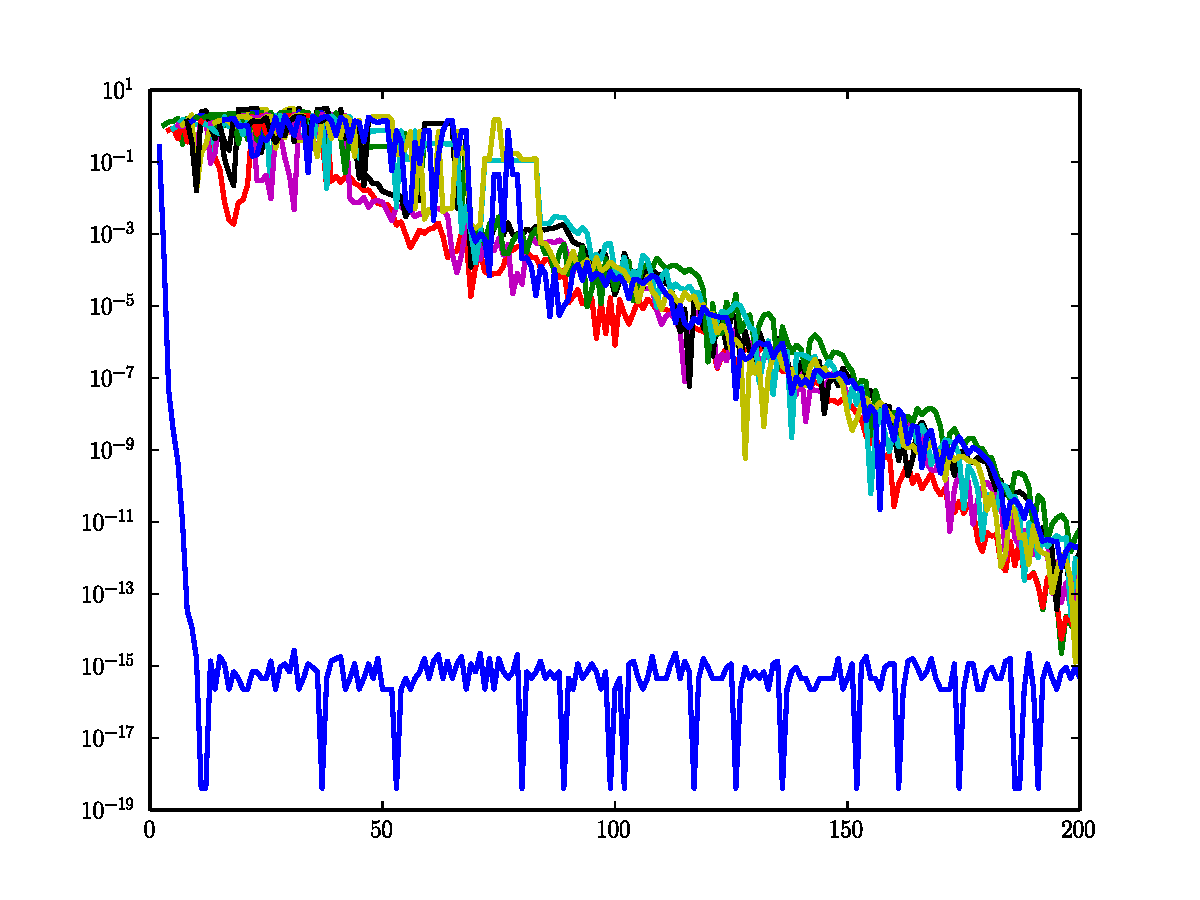
\includegraphics[width=\textwidth]{figures/rand_vals_conv.pdf}
    \caption{The blue line plots the error of the Ritz value of largest magnitude.
    This eigenvalue converges after fewer than 20 iterations}
    \label{fig:arnoldi_random_val_conv}
\end{subfigure}
\begin{subfigure}[b]{.49\textwidth}
    \centering
    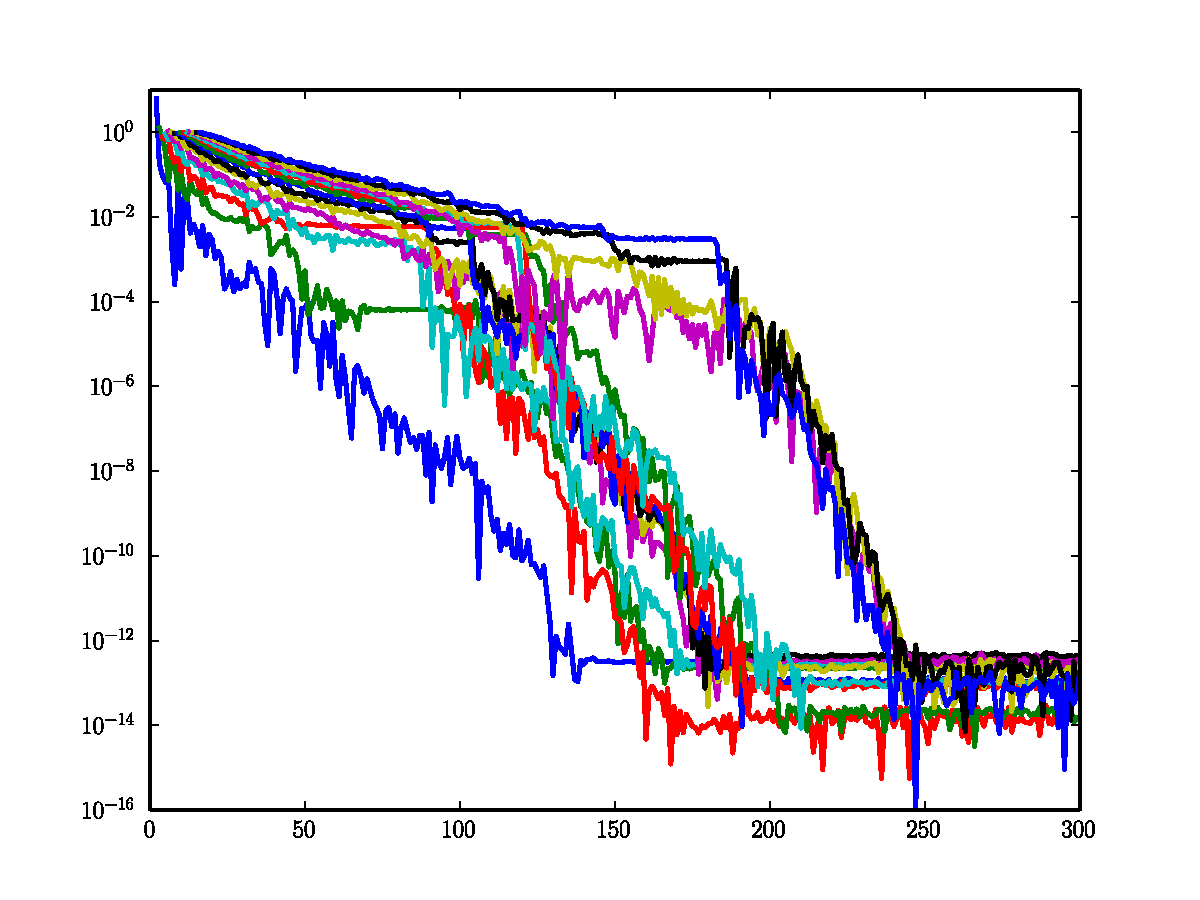
\includegraphics[width=\textwidth]{figures/rand_eigs_conv.pdf}
    \caption{All Ritz values have roughly equivalent magnitude.
    They take from 150 to 250 iterations to converge. }
    \label{fig:arnoldi_random_eig_conv}
\end{subfigure}
\caption{These plots show the relative error of the Ritz values as approximations to the eigenvalues of a matrix.
The figure at left plots the largest 15 Ritz values for a $500\times 500$ matrix with random entries.
The figure at right plots the largest 15 Ritz values for a $500\times 500$ matrix with uniformly distributed eigenvalues.}
\end{figure}

% TODO: this problem may be too difficult.
\begin{problem}
Finish the following function to visualize the convergence of the Ritz values.

\begin{lstlisting}
def plot_ritz(A, n, iters):
    """Plot the relative error of the Ritz values of `A'. Use the number of
    iterations as the x-axis and the relative error of the Ritz values of H_k
    a approximations to the eigenvalues of A as the y-axis.

    Inputs:
        A (ndarray)
        n (int): The number of Ritz values to plot.
        iters (int): The number of times to perform the Arnoldi iteration.
    """
    \end{lstlisting}

If $\tilde{\x}$ is an an approximation to $\x$, then the \emph{absolute error} in the approximation is
\[
\frac{\|\x - \tilde{\x}\|}{\|\x\|}.
\]
Hint: The most difficult part of this problem is to identify which Ritz values correspond to which eigenvalues.
After finding the Ritz values (or eigenvalues) of largest magnitude, use \li{np.sort()} to put them in order.
Make sure that this order is preserved throughout your program.

It may help to use the following algorithm.
\begin{enumerate}
    \item Find $n$ eigenvalues of $A$ of largest magnitude. Store these in order.
    \item Create an empty array to store the relative errors. For every $k \in $\li{[1, iters)},
    \begin{enumerate}
        \item Compute $H_k$ with the Arnoldi iteration.
        \item Find $n$ eigenvalues of $A$ of largest magnitude. Note that for small $k$, the matrix $H_k$ may not have this many eigenvalues.
        \item Store the absolute error. Make sure that the errors are stored in the correct order. For small $k$, some entries in the row or column may not be used.
    \end{enumerate}
    \item Use array broadcasting to compute the absolute error.
    \item Iteratively plot the errors. Lines for distinct eigenvalues should start at different places on the x-axis.
\end{enumerate}

Run your function on these examples.
The plots should be fairly similar to Figures \ref{fig:arnoldi_random_eig_conv} and \ref{fig:arnoldi_random_val_conv}.

\begin{lstlisting}
>>> # A matrix with random entries
>>> A = np.random.rand(300, 300)
>>> plot_ritz(A, 10, 175)
>>>
>>> # A matrix with uniformly distributed eigenvalues
>>> D = np.diag(np.random.rand(300))
>>> B = A.dot( D.dot(la.inv(A)) )
>>> plot_ritz(B, 10, 175)
\end{lstlisting}

If your code takes too long to run, consider integrating your solutions to Problems \ref{prob:arnoldi} and \ref{prob:ritz} with the body of this function.
\end{problem}

% Once the eigenvalue lab has been rewritten, have them use their own solver to find the eigenvalues of the $H_k$.

% This problem is very ill-conditioned.
\begin{comment}
\begin{problem}
Finding the roots of a polynomial can be represented as an eigenvalue problem.
Finding the roots of a monic polynomial (a polynomial with leading coefficient 1) $p = c_0 + c_1 x + \dots + c_{n-1} x^{n-1} + x^n$ is equivalent to finding the eigenvalues of the matrix
\[C = \begin{bmatrix}
0 & 0 & \dots & 0 & -c_0 \\
1 & 0 & \dots & 0 & -c_1 \\
0 & 1 & \dots & 0 & -c_2 \\
\vdots & \vdots & \ddots & \vdots & \vdots \\
0 & 0 & \dots & 1 & -c_{n-1} \end{bmatrix}\]
This matrix is called the companion matrix of the polynomial $p$.
As it happens, every matrix is similar to the companion matrix of its characteristic polynomial, but we won't use that fact here.

The following is a function that, given an array containing the coefficients $c_0, c_1, \dots, c_{n-1}$ for a monic polynomial $p$, performs matrix multiplication by the corresponding companion matrix.

\begin{lstlisting}
def companion_multiply(c, u):
    v = np.empty_like(u)
    v[0] = - c[0] * u[-1]
    v[1:] = u[:-1] - c[1:] * u[-1]
    return v
\end{lstlisting}

Use the Arnoldi iteration to estimate the five zeros of largest norm of a degree $1000$ monic polynomial with randomly chosen coefficients (the leading coefficient still needs to be 1).
Run $50$ steps of the Arnoldi iteration.
Compare your results with the roots of the polynomial computed using NumPy's \li{poly1d} class.
This computation can be done like this (where \li{c} is the array of random coefficients for the polynomial)

\begin{lstlisting}
p = np.poly1d([1] + list(c[::-1]))
roots = p.roots
# Now sort by absolute value from largest to smallest
roots = roots[np.absolute(roots).argsort()][::-1]
\end{lstlisting}

How close are the first few zeros of largest norm?
\end{problem}
\end{comment}

\section*{Lanczos Iteration (Optional)} % =====================================

The Lanczos iteration is a version of the Arnoldi iteration that is optimized to operate on symmetric matrices.
If A is symmetric, then \eqref{equ:hqa} shows that $H_k$ is symmetric and hence tridiagonal.
This leads to two simplifications of the Arnoldi algorithm.

First, we have $0=H_{k, n}=\langle \q_k, A\q_n \rangle$ for $k \leq n-2$; i.e., $A\q_n$ is orthogonal to $\q_1, \ldots, \q_{n-2}$.
Thus, if the goal is only to compute $H_k$ (say to find the Ritz values), then we only need to store the two most recently computed columns of $Q$.
Second, the data of $H_k$ can also be stored in two vectors, one containing the main diagonal and one containing the first subdiagonal of $H_k$.
(By symmetry, the first superdiagonal equals the first subdiagonal of $H_k$.)

The Lanczos iteration is found in Algorithm \ref{alg:lanczos_iteration}.

\begin{algorithm}
\begin{algorithmic}[1]
\Procedure{Lanczos}{$\b, A, k, tol$}
	\State $\q_0 \gets \zeros{\size{\b}}$								\Comment{Some initialization}
	\State $\q_1 \gets \b/\norm{\b}_2$
	\State $\x \gets \allocate{k}$
	\State $\y \gets \allocate{k}$
	\For{$i=0\ldots k-1$}									\Comment{Perform the iteration.}
		\State $\z \gets A\q_1$					\Comment{$\z$ is a temporary vector to store $\q_{i+1}$.}
		\State $\x[i] \gets \q_1\trp \z$				\Comment{$\q_1$ is used to store the previous $\q_i$.}
		\State $\z \gets \z - \x[i] \q_1 + \y[i-1] \q_0$				\Comment{$\q_0$ is used to store $\q_{i-1}$.}
		\State $\y[i] = \norm{\z}_2$						\Comment{Initialize $\y[i]$.}
		\If{$\y[i]<tol$}								\Comment{Stop if $\norm{ \q_{i+1}}_2$ is too small.}
			\State \pseudoli{return} $\x[: i+1]$, $\y[: i]$
		\EndIf
		\State $\z = \z/ \y[i]$
		\State $\q_0, \q_1 = \q_1, \z$						\Comment{Store new $\q_{i+1}$ and $\q_i$ on top of $\q_1$ and $\q_0$.}
	\EndFor
	\State \pseudoli{return} $\x$, $\y[: -1]$
\EndProcedure
\end{algorithmic}
\caption{The Lanczos Iteration. This algorithm operates on a vector $\b$ of length $n$ and an $n \times n$ symmetric matrix $A$. It iterates $k$ times or until the norm of the next vector in the iteration is less than $tol$. It returns two vectors $\x$ and $\y$ that respectively contain the main diagonal and first subdiagonal of the current Hessenberg approximation.}
\label{alg:lanczos_iteration}
\end{algorithm}

\begin{problem}
\label{prob:lanczos}
Implement Algorithm \ref{alg:lanczos_iteration} by completing the following function.
Write it so that it can operate on complex arrays.
\begin{lstlisting}
def lanczos(b, Amul, k, tol=1E-8):
    '''Perform `k' steps of the Lanczos iteration on the symmetric linear
    operator defined by `Amul', starting with the vector 'b'.

    INPUTS:
    b    - A NumPy array. The starting vector for the Lanczos iteration.
    Amul - A function handle. Should describe a symmetric linear operator.
    k    - Number of times to perform the Lanczos iteration.
    tol  - Stop iterating if the next vector in the Lanczos iteration has
          norm less than `tol'. Defaults to 1E-8.

    RETURN:
    Return (alpha, beta) where alpha and beta are the main diagonal and
    first subdiagonal of the tridiagonal matrix computed by the Lanczos
    iteration.
    '''
\end{lstlisting}
\end{problem}

As it is described in Algorithm \ref{alg:lanczos_iteration}, the Lanczos iteration is not stable.
Roundoff error may cause the $\q_i$ to be far from orthogonal.
In fact, it is possible for the $\q_i$ to be so adulterated by roundoff error that they are no longer linearly independent.
% If needed we could make a separate lab on the Lanczos iteration and the Implicitly Restarted Lanczos Method.
% There isn't time or space here for it though.

\begin{problem}
The following code performs multiplication by a tridiagonal symmetric matrix.

\begin{lstlisting}
def tri_mul(a, b, u):
   ''' Return Au where A is the tridiagonal symmetric matrix with main
   diagonal a and subdiagonal b.
   '''
    v = a * u
    v[:-1] += b * u[1:]
    v[1:] += b * u[:-1]
    return v
\end{lstlisting}

Let $A$ be a $1000\times 1000$ symmetric tridiagonal matrix with random values in its nonzero diagonals.
Use the function \li{lanczos()} from Problem \ref{prob:lanczos} with 100 iterations to estimate the 5 eigenvalues of $A$ of largest norm.
Compare these to the 5 largest true eigenvalues of $A$

If you do this problem for different vectors $a$ and $b$, you may notice that occasionally the largest Ritz value is repeated.
This happens because the vectors used in the Lanczos iteration may not be orthogonal.
These erroneous eigenvalues are called ``ghost eigenvalues."
%They generally converge to actual eigenvalues of the matrix and can make the multiplicity of an eigenvalue look higher than it really is.
\end{problem}

There are modified versions of the Lanczos iteration that are numerically stable.
One of these, the Implicitly Restarted Lanczos Method, is found in SciPy as the function \li{scipy.sparse.linalg.eigsh()}.

\begin{comment}
\begin{problem}
In Lab \ref{lab:MarkovGraph} we discussed how to find the Laplacian Matrix of a graph.
The second-smallest eigenvalue of a graph is known as the ``Fiedler Value" or the ``algebraic connectivity."
The algebraic connectivity of a graph is positive if the graph is connected and zero if it is not.
In general, the multiplicity of the eigenvalue $0$ in the Laplacian matrix of a graph is the number of connected components of that graph.
The following code constructs the Laplacian matrix of a graph composed of a line of nodes.
The matrix is stored in \li{dia_matrix} format.

\begin{lstlisting}
from scipy import sparse
m = 1000
d = np.ones(m)
d[1:-1] += np.ones(m-2)
l = sparse.diags([-np.ones(m-1), d, -np.ones(m-1)], [-1, 0, 1])
\end{lstlisting}

Use the \li{eigsh} function to verify that this graph is connected.
You should look at documentation for the \li{scipy.sparse} library and find the options you need to use.
For proper convergence you will want to leave the number of eigenvalues computed at its default value.

The following code constructs the Laplacian matrix the same graph as before except that a single edge has been removed.

\begin{lstlisting}
m = 1000
cut = 500
d = np.ones(m)
d[1:-1] += np.ones(m-2)
d1 = -np.ones(m-1)
d1[cut] = 0
d[[cut, cut+1]] =1
l = sparse.diags([d1, d, d1], [-1, 0, 1])
\end{lstlisting}

Verify that this graph is not connected.
\end{problem}
\end{comment}
